\chapter{Estudio teórico}
\label{cap:Estudio teórico}
En este capítulo se presenta de forma resumida toda la información que se analizó en el proceso de investigación para encontar las herramientas adecuadas para llevar a cabo nuestros objetivos. Por un lado, se presentan las distintas herramientas de procesamiento del lenguaje y diferentes APIs de generación del lenguaje. Por otro lado, las diferentes herramientas para la generación de interfaces y almacenamiento de la información que se han llevado a cabo para desarrollar este proyecto. En el repositorio de github, además de las que han sido utilizadas en la versión final, se puede ver la instalación y el uso de algunas de las siguientes apis, librerías y herramientas que fueron probadas para ver sus limitaciones y decantarse por unas u otras. 
\section{Bibliotecas de Procesamiento del Lenguaje en Python}
\subsection{NLTK}
%https://www.nltk.org/
%Bird, Steven, Edward Loper and Ewan Klein (2009), Natural Language Processing with Python. O’Reilly Media Inc.
La biblioteca NLTK (Natural Language Toolkit) ofrece una amplia gama de herramientas y recursos para tareas de PLN.

En primer lugar, NLTK permite realizar tareas como la tokenización y el  etiquetado POS (Part-Of-Speech tagging). Al utilizar las herramientas de tokenización, podemos dividir el texto en unidades más pequeñas, lo que facilita el análisis y la comprensión. El etiquetado POS asigna etiquetas gramaticales a cada palabra en el texto, lo que nos permite identificar la función de cada palabra en la oración. 

\begin{lstlisting}[style=SpyderStyle, caption={Ejemplo de código en Python}, captionpos=b, label={lst:python},breaklines = true]
	sentence = "Reminiscence Therapy involves the discussion of past activities using prompts like photos."
	tokens = nltk.word_tokenize(sentence)
	tagged = nltk.pos_tag(tokens)
	tagged[0:len(tagged)]
\end{lstlisting}

En este código $nltk$ tokeniza la oración introducida y etiqueta cada $token$ indicando la categoría sintáctica de cada $token$ como sigue:

\begin{itemize}
	\item NNP: Nombre propio singular
	\item NN: Nombre, singular o sustantivo singular
	\item VBZ: Verbo tercera persona del singular presente
	\item DT: Determinante
	\item IN: Preposición o oración subordinada
	\item JJ: Adjetivo
	\item NNS: Nombre plural 
	\item VBG: Verbo, gerundio o participio
	\item . : Signo de puntuación
\end{itemize}

\begin{lstlisting}[style=SpyderStyle, caption={Tokenización y etiquetado con nltk}, captionpos=b, label={lst:python},breaklines = true]
>>[('Reminiscence', 'NNP'), ('Therapy','NNP'), ('involves','VBZ'), ('the', 'DT'), ('discussion', 'NN'), ('of', 'IN'), ('past', 'JJ'), ('activities', 'NNS'), ('using', 'VBG'), ('prompts', 'NNS'), ('like', 'IN'), ('photos', 'NNS'), ('.', '.')]

\end{lstlisting}

Otras de las funcionalidades que nos permite esta biblioteca es el análisis sintáctico o lematización. Por ejemplo, nos permite la obtención de árboles sintácticos, lo que permite visualizar la estructura gramatical de las oraciones, facilita el análisis y la interpretación del texto. \\

\begin{figure}[h]
	\centering
	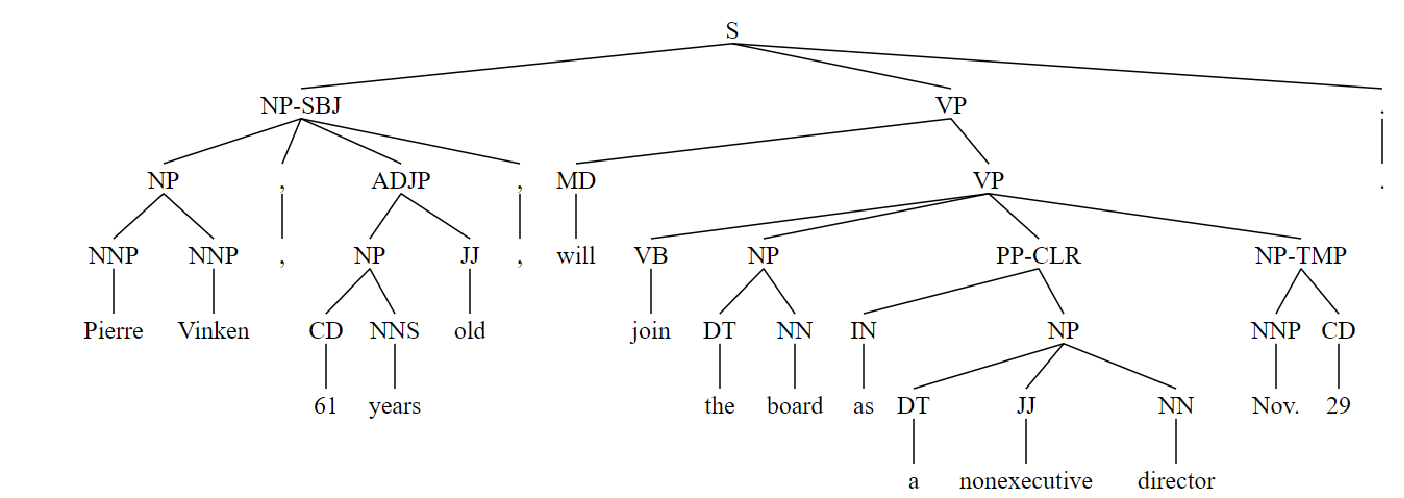
\includegraphics[width=0.9\textwidth]{Imagenes/arbolsintactico}
	\caption{Árbol sintáctico generado con nltk}
	\label{fig:1}
\end{figure}

\begin{lstlisting}[style=SpyderStyle, caption={Análisis sintáctico y lematización con nltk}, captionpos=b, label={lst:python},breaklines = true]
entities = nltk.chunk.ne_chunk(tagged)
nltk.download('treebank')
from nltk.corpus import treebank
t = treebank.parsed_sents('wsj_0001.mrg')[0]
t
\end{lstlisting}


Además de estas características fundamentales, NLTK ofrece una serie de otras funcionalidades que amplían aún más su utilidad. Por ejemplo, incluye herramientas para la extracción de entidades nombradas, el análisis de sentimientos, la generación de texto y la traducción automática. Estas capacidades adicionales permiten abordar una amplia variedad de tareas en el procesamiento del lenguaje natural, desde la clasificación de texto hasta la generación de resúmenes automáticos y la traducción de idiomas. En resumen, NLTK es una herramienta invaluable para investigadores, estudiantes y profesionales que trabajan en el campo del PLN, ofreciendo una amplia gama de funcionalidades que facilitan el análisis, la comprensión y la manipulación del lenguaje humano.


\subsection{SpaCy}

spaCy es una biblioteca de procesamiento del lenguaje natural diseñada para ser rápida, eficiente y fácil de usar. Ofrece herramientas para realizar tareas de PLN como tokenización, análisis sintáctico, reconocimiento de entidades nombradas y más. spaCy se destaca por su velocidad y rendimiento, lo que la hace ideal para aplicaciones que requieren procesamiento de texto a gran escala, como el análisis de grandes volúmenes de datos o el procesamiento en tiempo real.

Una de las principales ventajas de spaCy es su modelo de lenguaje pre-entrenado, que permite a los usuarios comenzar a trabajar con PLN de inmediato sin necesidad de entrenar modelos desde cero. Además, spaCy ofrece una API fácil de usar y una documentación exhaustiva que facilita su aprendizaje y su integración en proyectos. Sin embargo, debido a su enfoque en la velocidad y la eficiencia, spaCy puede carecer de ciertas funcionalidades más avanzadas que otras bibliotecas ofrecen.

\subsection{Gensim}

Gensim es una biblioteca de PLN especializada en modelado de temas y procesamiento de texto a gran escala. Ofrece herramientas para construir, entrenar y utilizar modelos de vectores de palabras (word embeddings), modelos de espacio vectorial, y modelos de temas para analizar grandes colecciones de texto. Gensim se destaca por su eficiencia y su capacidad para manejar grandes conjuntos de datos de texto de manera rápida y efectiva.

Una de las principales ventajas de Gensim es su enfoque en el modelado de temas, que permite a los usuarios descubrir patrones y estructuras ocultas en grandes corpus de texto. Además, Gensim ofrece una API intuitiva y fácil de usar, así como una variedad de algoritmos de modelado de temas y similitud de documentos. Sin embargo, Gensim puede requerir cierto conocimiento previo de PLN y estadística para utilizarlo de manera efectiva, y puede carecer de algunas funcionalidades más generales de PLN que otras bibliotecas ofrecen.

\subsection{TextBlob}

TextBlob es una biblioteca de PLN que proporciona una interfaz sencilla para realizar tareas comunes de procesamiento del lenguaje natural, como tokenización, etiquetado POS, análisis de sentimientos y más. Está construida sobre NLTK y Pattern, dos bibliotecas populares de PLN en Python, lo que le permite aprovechar sus funcionalidades mientras simplifica su uso con una API más amigable para los usuarios.

Una de las principales ventajas de TextBlob es su facilidad de uso y su API intuitiva, que permite a los usuarios realizar tareas de PLN con solo unas pocas líneas de código. Además, TextBlob ofrece modelos pre-entrenados para el análisis de sentimientos y la corrección ortográfica, lo que facilita el desarrollo de aplicaciones de PLN sin necesidad de entrenar modelos desde cero. Sin embargo, debido a su enfoque en la simplicidad y la facilidad de uso, TextBlob puede carecer de algunas funcionalidades más avanzadas que otras bibliotecas ofrecen.

\subsection{Transformers}

Transformers es una biblioteca de PLN basada en la arquitectura de atención, que ha demostrado ser muy eficaz en una variedad de tareas de PLN, como modelado de lenguaje, traducción automática, y más. Ofrece una amplia gama de modelos pre-entrenados, como BERT, GPT y T5, que han establecido nuevos estándares de rendimiento en muchas tareas de PLN. Transformers se destaca por su capacidad para capturar relaciones semánticas complejas y su flexibilidad para adaptarse a diferentes dominios y lenguas.

Una de las principales ventajas de Transformers es su estado del arte en rendimiento, que ha superado a muchas otras bibliotecas y enfoques de PLN en una variedad de tareas. Además, Transformers ofrece una API fácil de usar y una variedad de modelos pre-entrenados listos para usar, lo que facilita su integración en proyectos de PLN. Sin embargo, debido a su complejidad y su enfoque en modelos de última generación, Transformers puede requerir recursos computacionales significativos y puede ser más difícil de entender y utilizar para usuarios principiantes en PLN.

\section{APIs de procesamiento del lenguaje}

Las APIs de procesamiento del lenguaje son conjuntos de herramientas y servicios que permiten a los desarrolladores integrar capacidades de procesamiento del lenguaje natural (NLP) en sus aplicaciones y sistemas. Estas APIs ofrecen funcionalidades como análisis de sentimientos, reconocimiento de entidades nombradas, etiquetado de partes del discurso, traducción automática, resumen de texto, entre otros. Al utilizar una API de procesamiento del lenguaje, los desarrolladores pueden aprovechar las capacidades avanzadas de NLP sin necesidad de desarrollar desde cero sus propios algoritmos y modelos. Esto facilita la implementación de características de procesamiento del lenguaje en una amplia variedad de aplicaciones, desde chatbots hasta análisis de redes sociales y sistemas de recomendación.

Las APIs modernas suelen contar con todas las funcionalidades que contaban las bibliotecas de Python mencionadas anteriormente. En concreto, para el desarrollo de este proyecto se estudiaron las APIs que se presentan a continuación.

\subsection{Bard}
Bard es una API de procesamiento del lenguaje natural creada por Google, diseñada para ofrecer respuestas conversacionales a través de interacciones de mensajes. Basada en LaMDA, un modelo de lenguaje experimental de Google, Bard se enfoca en proporcionar respuestas coherentes y relevantes a preguntas realizadas en lenguaje natural.

Esta inteligencia artificial compite directamente con ChatGPT y ChatGPT Plus, con el objetivo de ofrecer una alternativa propia en el campo del procesamiento del lenguaje natural. Al igual que sus competidores, Bard permite realizar consultas y recibir respuestas sin necesidad de navegar por diferentes páginas web.

En su desarrollo, Google ha priorizado la accesibilidad y la transparencia, ofreciendo modelos y recursos de PLN de código abierto que pueden ser utilizados y modificados por la comunidad. Bard se basa en el modelo LaMDA, anteriormente en fase de pruebas cerradas, pero ahora disponible para un público más amplio.

LaMDA, que significa "Language Model for Dialogue Applications", ha sido rebautizado como Bard para su lanzamiento oficial. Inicialmente, Bard se lanzará con un modelo reducido de LaMDA, lo que permitirá su uso por parte de más usuarios y facilitará la obtención de comentarios para su mejora continua.

En diciembre de 2023, Google fortaleció la capacidad de Bard al incorporar Gemini Pro en inglés, brindando habilidades más avanzadas de comprensión, razonamiento, resumen y codificación. Posteriormente, en febrero de 2024, se anunció la expansión de Gemini Pro a más de 40 idiomas y se oficializó el cambio de nombre de Bard a Gemini, con lo que se tuvo que descartar el primer modelo del proyecto desarrollado en Bard, y tampoco se pudo volcar a Gemini ya que, por el momento, no está disponible en España. 
\subsection{Gemma}

Gemma es una API de PLN desarrollada por OpenAI. Utiliza modelos de lenguaje basados en la arquitectura GPT (Generative Pre-trained Transformer) para una variedad de tareas de PLN, como generación de texto, análisis de sentimientos, clasificación de texto, y más. Gemma se destaca por su capacidad para generar texto coherente y de alta calidad en una variedad de estilos y tonos, así como por su facilidad de uso y su API intuitiva.

Una de las principales ventajas de Gemma es su rendimiento en tareas de generación de texto, donde ha establecido nuevos estándares de calidad y coherencia en muchos casos. Además, Gemma ofrece modelos pre-entrenados en varios dominios y lenguas, lo que facilita su integración en una variedad de aplicaciones de PLN. Sin embargo, debido a su enfoque en modelos de última generación, Gemma puede requerir recursos computacionales significativos y puede ser más difícil de entender y utilizar para usuarios principiantes en PLN.


En primer lugar, estos modelos se trabajaron en Google Collaborate aumentando el número de GPUs. De esta forma gemma tiene un buen comportamiento y genera respuestas adecuadas y coherentes. En concreto, una respuesta generada por \textit{gemma-7b} sería la siguiente.
\begin{center}
	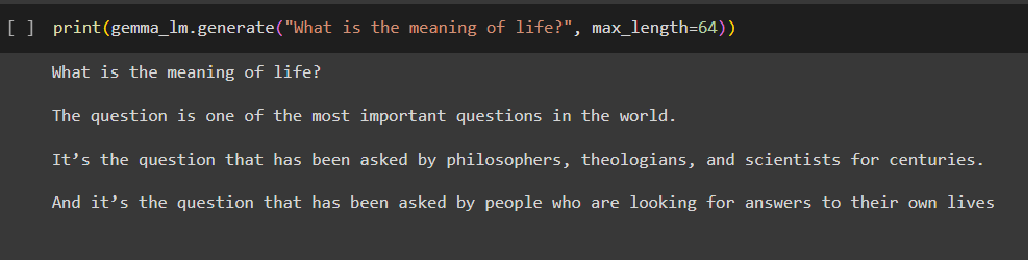
\includegraphics[width=0.75\textwidth]{Imagenes/gemma (1)}
\end{center}
Sin embargo, las limitaciones propias de Google Collaborate no permitían en la versión gratuita aumentar el número de GPUs de forma frecuente y en consecuencia tuve que estudiar el modelo en otro entorno. Para ejecutarlo de forma local y obtener un buen comportamiento es necesario instalar Linux y descargar el modelo de Hugging face. 

Aunque \textit{gemma-2b} en la versión local instalada desde Hugging Face en Linux tiene un buen comportamiento, genera respuestas incoherentes que hacen de este modelo poco útil para nuestro proyecto. La versión \textit{gemma-7b} genera respuestas mucho mejores pero tiene la enorme desventaja de que ocupa una gran cantidad de espacio en memoria.

\subsection{GPT API}

GPT API es una API de PLN desarrollada por OpenAI. Utiliza modelos de lenguaje basados en la arquitectura GPT (Generative Pre-trained Transformer) para una variedad de tareas de PLN, como generación de texto, análisis de sentimientos, clasificación de texto, y más. GPT API se destaca por su capacidad para generar texto coherente y de alta calidad en una variedad de estilos y tonos, así como por su facilidad de uso y su API intuitiva.

Una de las principales ventajas de GPT API es su rendimiento en tareas de generación de texto, donde ha establecido nuevos estándares de calidad y coherencia en muchos casos. Además, GPT API ofrece modelos pre-entrenados en varios dominios y lenguas, lo que facilita su integración en una variedad de aplicaciones de PLN. Sin embargo, debido a su enfoque en modelos de última generación, GPT API puede requerir recursos computacionales significativos y puede ser más difícil de entender y utilizar para usuarios principiantes en PLN.

Sin embargo para obtener el comportamiento que se necesitaba en este trabajo debía ser entrenada, y debido a las limitaciones hardware esto suponía una cantidad de tiempo inviable. 

\subsection{Rasa}
Entre las opciones que se barajaron para seguir desarrollando el proyecto se encuentra Rasa. Rasa es una plataforma de código abierto diseñada para el desarrollo de chatbots y asistentes virtuales conversacionales. Utilizando técnicas de procesamiento de lenguaje natural (NLP) y aprendizaje automático, Rasa permite a los desarrolladores crear sistemas de diálogo inteligentes y personalizados. Una de las principales ventajas de Rasa es su flexibilidad y personalización, ya que los desarrolladores tienen control total sobre el comportamiento y la lógica de sus chatbots. Además, Rasa proporciona herramientas robustas para la gestión del diálogo, la comprensión del lenguaje natural y la integración con otros sistemas. Sin embargo, una posible desventaja de Rasa es su curva de aprendizaje, ya que requiere un conocimiento sólido de NLP y aprendizaje automático para aprovechar al máximo su potencial. Además, debido a su naturaleza de código abierto, puede requerir más tiempo y recursos para implementar y mantener en comparación con otras soluciones comerciales. Sin embargo, aunque rasa no es la api más potente en cuánto a generación de texto, tiene numerosas aplicaciones que resultan interesantes. Por ejemplo, gracias a la api de rasa es fácil volcar la interfaz de código en Python sobre la interfaz de Telegram. 

\subsection{Gemini}

%De aqui quiero sacar varias páginas, ver el tutorial y ir metiendo todo

Gemini es una API de PLN desarrollada por Google. Utiliza modelos de lenguaje basados en la arquitectura Transformer para una variedad de tareas de PLN, como análisis de sentimientos, extracción de entidades, traducción automática, y más. Gemini se destaca por su rendimiento en tareas de procesamiento de texto, donde ha demostrado superar a muchas otras APIs y enfoques de PLN en términos de precisión y velocidad.

Una de las principales ventajas de Gemini es su capacidad para manejar grandes volúmenes de texto de manera eficiente y efectiva. Además, ofrece una API fácil de usar que permite a los desarrolladores integrar fácilmente capacidades de PLN en sus aplicaciones. Sin embargo, debido a su enfoque en el rendimiento y la eficiencia, Gemini puede carecer de algunas funcionalidades más avanzadas que otras APIs ofrecen.

Finalmente, se decidio utilizar la API de Gemini descartada en un primer momento por no estar disponible en España. Por tanto, para su uso, y en consecuencia para hacer funcionar el proyecto es necesario tener una VPN conectada a uno de los países en los que Gemini esta disponible. Una vez conectado se ha de obtener una API KEY y configurar el proyecto adecuadamente. Durante el resto de uso del programa, sigue siendo necesario estar conectado a la VPN.

%No sé incluso si no hacerlo un propio cápitulo de la elección de API ya que ha sido 3 meses dedicado a la investigación de qué api usar


%Pasar todas las APIs de las que se hablo en el otro sitio 

%Hablar de las VPN y de la aplicación que se ha usado para eso mismo

%Finalmente poner capturas de consultas a la api de gemini, la estructura de las respuestas, analizar los diferentes modelos, decir porque se ha elegido gemini pro


%Decir ventajas poniendo capturas de preguntas y respuestas que da gemini 
%También hablar de las limitaciones 
\section{Almacenamiento de la información}	
\subsection{JSON}
El uso de objetos JavaScript (JSON) es una poderosa herramienta de programación. Ya sea para almacenar datos o crear una API, convertir sus datos en JSON los hace reutilizables, independientemente de la tecnología que acceda a ellos. La diferencia entre un objeto JSON y un diccionario de Python es mínima, por lo tanto, es fácil almacenar un diccionario de Python como JSON utilizando la biblioteca del analizador json. Las ventajas de utilizar JSON para almacenar información radican en su legibilidad humana, ligereza en términos de uso de recursos y tamaño de almacenamiento, flexibilidad para representar una variedad de estructuras de datos, interoperabilidad entre diferentes sistemas y lenguajes de programación, y su fácil manejo en entornos como Python, donde se pueden mapear directamente a diccionarios, facilitando así el procesamiento y manipulación de datos en aplicaciones. Unificar toda esta información permite una comprensión clara y completa de las ventajas y usos de JSON en el almacenamiento de datos y la comunicación entre sistemas.

\subsection{RDF}

%Las tripletas RDF (Resource Description Framework) son una estructura de datos fundamental en la web semántica para representar información en forma de sujetos, predicados y objetos. Cada tripleta consiste en un sujeto que es una entidad, un predicado que describe la relación entre el sujeto y el objeto, y un objeto que puede ser una entidad o un valor. Por ejemplo, en la tripleta "Gato - es_un - Animal", "Gato" es el sujeto, "es_un" es el predicado y "Animal" es el objeto.

Estas tripletas RDF se utilizan para almacenar información de manera estructurada y semántica, lo que permite una representación más rica y significativa de los datos en la web. A través de vocabularios y ontologías, como RDF Schema (RDFS) y Web Ontology Language (OWL), se establecen relaciones y significados precisos entre los términos utilizados en las tripletas RDF.

Las tripletas RDF son ampliamente utilizadas en la web semántica para diversas aplicaciones, como la descripción de recursos y metadatos en la web, la integración de datos de diferentes fuentes, la creación de motores de búsqueda más inteligentes y la construcción de sistemas de recomendación personalizados. Además, RDF proporciona un marco estándar y flexible para representar conocimiento y facilita la interoperabilidad entre diferentes sistemas y aplicaciones en la web.

\section{Bibliotecas para el desarrollo de interfaces}

PyQt, wxPython y Kivy son opciones populares para la implementación de interfaces gráficas, cada una con sus propias ventajas y desventajas.

PyQt es conocido por su completo conjunto de widgets, lo que te permite crear interfaces gráficas complejas y altamente personalizadas. Sin embargo, puede tener una curva de aprendizaje más pronunciada debido a su complejidad y sintaxis más verbosa.

Por otro lado, wxPython ofrece una sintaxis más simple y fácil de entender, lo que puede ser beneficioso si estás empezando o prefieres un enfoque más directo. Aunque tiene menos widgets y funcionalidades avanzadas que PyQt, sigue siendo una opción sólida con una comunidad activa que proporciona soporte.

Kivy destaca por su diseño adaptable, diseñado para crear aplicaciones con interfaces gráficas que funcionan en una amplia gama de dispositivos. Utiliza un lenguaje de marcado declarativo que permite definir la interfaz de usuario de manera intuitiva y separada del código Python. Sin embargo, puede tener menos documentación y recursos disponibles en comparación con PyQt y wxPython.







